% TODO for a $16\times 16$ segmentation patch there exist, in theory $2^256$ possible edge masks. Due to the inherent structure in image patches however, not all of them are likely, and those containing simple structures are prevalent.
% TODO put an image of decision of 4 trees in one pixel
\chapter{Capturing image edge structure} %Structured random decision forests}
\label{Chapter2}
\settocdepth{subsection}
Recently, very good edge detection results were achieved using random decision forests. In this chapter we discuss the recent edge detection works by Doll\'ar and Zitnick \cite{DollarICCV13edges,Dollar2015PAMI}. Their algorithm - Structured edge ({\bf SE}) takes a data-driven approach to learning of semantic edges. % Let the data speak for itself
%Their goal is
They manage to achieve accurate and fast edge detection. % real-time

By ``structure'' in image edges % as well as in SF leaves
we mean the fact that small %local 
image patches are known \cite{Ren2006figure,LimZD13} to show % exhibit
notable %prominent
forms of local structure (some examples in \fref{fig:srf-structure-in-edge-patches}). As edges are interdependent, often shapes like straight and curved lines, T-junctions and Y-junctions, convexities, sharp corners and parallel lines are to be observed in a local neighbourhood.

\textbf{Capturing more context:} A family of learning approaches have tried to leverage local context to organise images - discover image edges, or recognise %discern
figure from background objects. First the Boosted Edge Learning (BEL) algorithm~\cite{Dollar2006supervised} made at each location in the image an independent binary decision as to the presence or absence of image edge. Noticing the abundance of edge structure in a local patch, \textit{sketch tokens}~\cite{LimZD13} and \textit{shapemes}~\cite{Ren2006figure} organise local edge shapes by clustering. 
The Structured forest ({\bf SF})~\cite{DollarICCV13edges} takes this idea a step further and keeps all local segmentation patches it has seen at training time in the leaves of its decision trees. By abstaining from using pre-defined classes of edge patches, clustering, or averaging \textbf{to model local edge context}, the SF framework has the potential to learn subtle variations in edge structure. It is flexible - it is able to adapt to the training dataset at hand by letting the data speak for itself. That is one of the reasons for its highly accurate edge detection.

\textbf{Structured forest ``knows'' image edge context:} Precisely the ability of the structured forest to predict a local segmentation mask given an input image patch is so important to us. Even better, the edge detector SE could provide as a by-product the segmentation predictions that it has made at every image location. We would like to use this information in order to obtain image segmentation.

In this chapter we review the SE edge detector and elucidate why it is a good first-step choice for our task of semantic segmentation.

\section{Structured forests}
Structured random forests~\cite{KontschiederBBP11,DollarICCV13edges} is a machine learning algorithm, an extension of random forests which allows the use of structured input data and\slash or the making of structured predictions.

\settocdepth{section} % avoid listing this in the toc, but give it a number in the text
\subsection{Random decision forests}
\settocdepth{subsection}
Random forest (RF) is a recently introduced~\cite{Breiman01} learning approach which has found applications in computer vision~\cite{KontschiederBBP11,LimZD13,DollarICCV13edges,Dollar2015PAMI} due to its speed both at training and testing time, high accuracy, and robustness to noise.

A random decision forest is a collection %an ensemble %a combination 
of tree predictors - classifiers or regressors~\cite{breiman1984classification}. Here ``tree'' is used in the computer science sense to denote an abstract data structure (ADS) - a graph without cycles. 
The predictive power of the forest depends on the strength of the individual trees and their de-correlation. To this end, %Therefore 
every tree is constructed based on a vector, sampled independently and randomly from the space of possible vectors. The randomness could be \wrt the training examples that are made available to each tree and\slash or the set of features that are being considered at each node of a decision tree.

Criminisi \etal~\cite{Criminisi12} provide a survey of decision tree methods.

Nowozin~\cite{Nowozin12improvedinformation,nowozin2014decision} discusses bias in the estimation of information gain for making split decisions at each node during decision tree training. He proposes estimators which lead to training better trees, yielding improved predictive performance.

\subsubsection{Structured learning}
By definition, {\bf structured learning} means that the input and output spaces can be arbitrarily complex. Examples are images, graphs, strings, bounding boxes, joints positions for object pose estimation, folds of proteins, sequences of actions. Among the initial methods proposed for the task of structured learning were probabilistic graphical models (PGMs) and structured support vector machines (structured SVMs).

\paragraph{Structured random forests}\mbox{}\\\mbox{}\\
\textbf{Structured forests for class labelling:} Kontschieder \etal \cite{KontschiederBBP11} were first to observe that RFs are applicable to the problem of structured learning. They remark that any type of input could be given to RF and they could preserve %conserve 
any type of output in the leaves of the trees. They extend the RF framework to work with structured class labels and use it to perform semantic image labelling (\textit{bike, cow, car, building, road \etc}).

\textbf{Structured forests for edge extraction:} In the rest of the current chapter %Next, 
we review the method of Doll{\'a}r and Zitnick \cite{DollarICCV13edges,Dollar2015PAMI} who apply Structured random decision forest to regular input (feature vectors obtained from image patches), but have ``structured'' output - they make local segmentation patch predictions.

\section{Structured edge algorithm outline}
The key to edge extraction using SF is that a decision for a single point is made based on an {\bf image patch centred at it}. A large enough patch contains low-level features as well as mid-level context information (see \fref{fig:srf-structure-in-edge-patches}). For improved accuracy, multiple patches (not just the one centred around the pixel) contribute to the final conclusion as to the presence or absence of an edge in the particular pixel. % decision

\begin{figure}[ht!]
\centering
 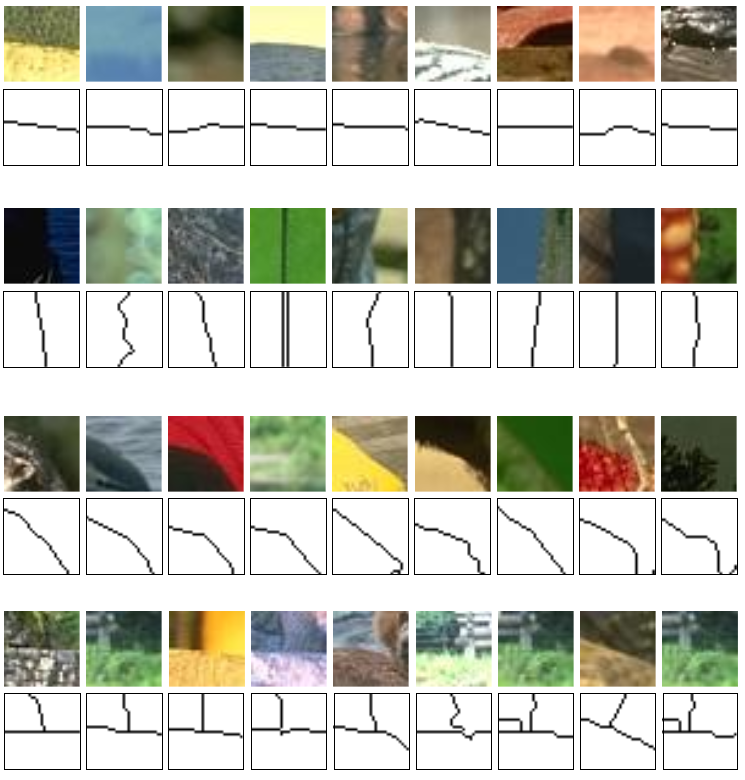
\includegraphics[width=0.5\textwidth]{images/srf/structure-in-edge-patches.png}
\caption[Local patches exhibit similarities in edge structure]{Local edge patches exhibit similarities in structure. Image patches and the human-%hand-
drawn edges present in them. Cropped from BSDS500, courtesy of \cite{DollarICCV13PresentationSlides}.}
\label{fig:srf-structure-in-edge-patches}
\end{figure}

SE is an example of supervised machine learning. During training time it is presented with patches and their ground truth annotations (local segmentations). It learns parameters that enable it to make predictions at testing time as to the most likely segmentation of fresh, {\bf unseen} so far {\bf patches}. For edge detection, it agglomerates those multiple patch decisions to obtain a probability of boundary ({\bf Pb} - see \fref{fig:sub:edge_detection-pb} and \fref{fig:sub:edge_detection-pb-cc}) - a probabilistic edge map for an entire image.

\section{Training - growing a decision forest}
A RF is trained by recursively growing its decision trees. 

\textbf{Input training data:} For the task of edge detection, the training data is a total of 1 million training samples. A training sample is a pair of an image patch and a corresponding to it ground-truth segmentation patch. Half of those are positive examples - a patch containing an edge and its hand-labelled segmentation. The other half are negative examples - so-called ``background patches'', their segmentation is trivial - a single class label on the whole patch, but the input patch contains important information that the SF would learn from. 

\textbf{Sifting the patches from the root down the tree:} To grow a decision tree means to learn what is a good way of redistributing the input data presented to the tree (at its root node) into its leaves. Such a distribution to the tree leaves would be good if in the end similar training samples are grouped together - in the same decision tree leaf. Notice that a ``perfect'' distribution of the patches would have each leaf contain a single patch. Such decision trees, however, overfit the training. In a trained structured decision tree, each leaf contains many patches, and all leaves contain patches.

In the following we discuss {\bf binary} decision trees, as this is the data structure used in practice by the SE algorithm. It is trivial to extend the algorithm to use general trees by making a multi-class decision at each node. 

% \textbf{Training is redistributing the data towards the leaves of a binary tree:} 
\subsection{Learning the split function}
\textbf{Pushing the patches down the tree is equivalent to learning how to split each inner node:} So at each node a binary decision must be made how to separate the training data into the left and right child sub-trees. Initially the root of the tree contains all training data available to the tree. A split function $h(x,\theta_j)\in\{0,1\}$ determines to which child an input training sample $x$ is forwarded. The parameter $\theta_j$ is what must be learnt for each node $j$ during training. A criterion based on {\bf information gain} is introduced to decide on optimal %good 
splits. Splitting is done in such a way so as to minimise entropy in the nodes. In this algorithm Gini impurity is used. Some of the improvements proposed by Nowozin~\cite{Nowozin12improvedinformation,nowozin2014decision} regarding entropy estimators are adopted in this work. Growing by splitting a node continues until either 1) a certain maximal tree depth is reached, or 2) sufficient purity of nodes is achieved.

The goal is to cluster in the leaves of the trained structured decision tree segmentation patches that correspond to input features which are as similar as possible. The nett effect is that similar segmentation patches should end up in the same leaf, see \fref{fig:structured-decision-tree-node-split}.

\settocdepth{section}
\subsection{Key contribution of the work}
\settocdepth{subsection}
The ``structured output'' in the case of the SE algorithm is a $d\times d$ segmentation patch (in practice they set $d = 16$). 
As the segmentation patch space is high-dimensional and complex, it is non-trivial to compute information gain in order to split the set of inputs into two subsets.

\textbf{Proxy label space:} They introduce a mapping to a simpler, lower-dimensional discrete space. The information gain computed on it is a sufficient approximation of that of the original output space without being prohibitively expensive to compute. Thus it is possible to compute distance, or, analogously, similarity, between output segmentation. In effect, similar output segmentations are clustered together.

\begin{figure}[ht!]
\centering
 \subfigure[A training sample is a pair of image patch and its corresponding ground-truth segmentation]{%
  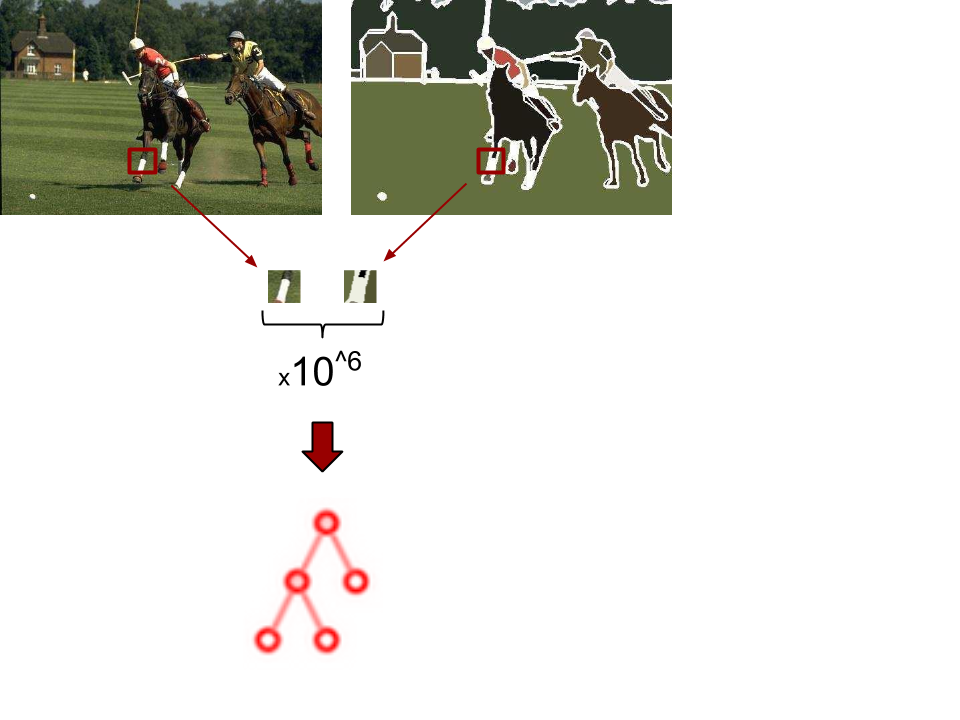
\includegraphics[width=0.5\textwidth]{images/srf/structured-decision-tree-training.png}
 }
 \subfigure[Splitting of training data at a node of a decision tree]{%
  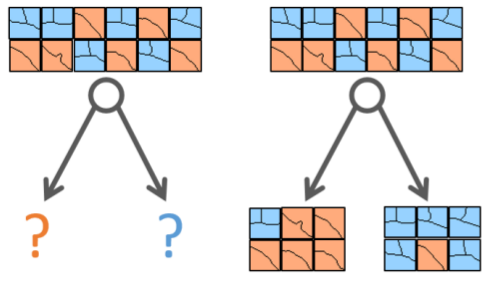
\includegraphics[width=0.3\textwidth]{images/srf/structured-decision-tree-node-split.png}
  \label{fig:structured-decision-tree-node-split}
 }
\caption[Training of a structured decision tree]{Training of a decision tree. \protect\subref{fig:structured-decision-tree-node-split} courtesy of \cite{DollarICCV13PresentationSlides}.}
\label{fig:srf-training}
\end{figure}

\settocdepth{section}
\subsection{Introducing randomness for diversity of the decision forest}
\settocdepth{subsection}
Part of the accuracy in prediction of the RF framework comes from ensuring sufficient diversity of trees. One way to achieve this, and how it is done in the SE algorithm, is by introducing randomness at each decision node. This is done by subsampling the input features that are taken into account when optimising the split at the tree node. SF achieves robust results by combining the output of $T$ decorrelated trees. Because of the small correlation of the trees in the ensemble, even small forests manage good performance - later we use SE with $T=4$.

\section{Inference}
Unlike other structured learning methods, no optimisation is required to make a prediction. Inference using SF is straightforward. A decision forest is an ensemble of $T$ \textit{independent} trees. To make a prediction, the individual predictions of the trees are combined as prescribed by the ensemble model. Here averaging is performed on the output edge patches.

\subsection{Structured decision tree inference}
The test sample - a feature vector computed based on an input image patch $x$, travels down the tree. Decisions whether it should be routed to the left or right child of a node are made according to the parameters learnt during training. When a leaf node is reached, it contains a set of most likely segmentations, and each of those could be associated with the input $x$.

\textbf{Ensemble model:} In the context of random forests the term ``ensemble model'' defines how to combine multiple predictions into a single prediction. Somewhat confusing, in the paper \cite{DollarICCV13edges}, this refers to two different things:
\begin{enumerate}
 \item{in {\bf decision tree inference:}} in order to associate a prediction with each leaf (like in \fref{fig:srf-tree-inference}). 
 To this end, the {\bf medoid} segmentation patch \textit{for the proxy output space} is chosen. This is the one that minimises the sum of distances to all others in the leaf patch, see \fref{fig:srf-leaf}. The medoid is the {\bf only patch} that is subsequently {\bf used}, out of all those patches that made it to the same tree leaf. 
 While during testing we get new input image patches, note that the {\bf predictions} for them can be only patches which have already been observed by the SF during training. % can be predicted during testing %by the SF % in this scenario.
 \item{in {\bf detection:}} to make the final edge extraction, a means of combining multiple overlapping decisions is necessary. Details will be given shortly in \sref{sec:ch2-edge-detection}.
\end{enumerate}

\begin{figure}[ht!]
\centering
 \subfigure[Image patches used as input, which ended up clustered in the same structured tree leaf.]{%
  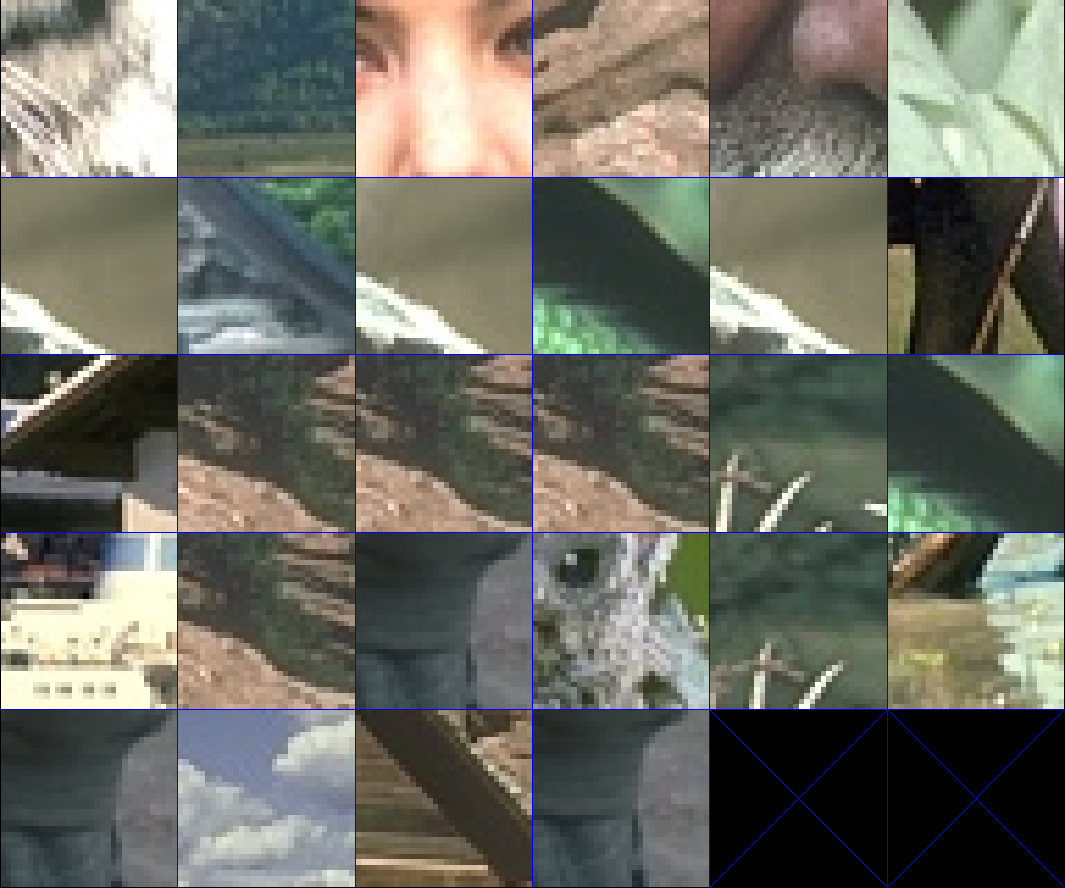
\includegraphics[width=0.45\textwidth]{images/srf/sf-leaf-imgs.png}
  \label{fig:sf-leaf-imgs}
 }
 \subfigure[Corresponding segmentation patches in a structured tree leaf. Upper left is the {\bf medoid}.]{%
  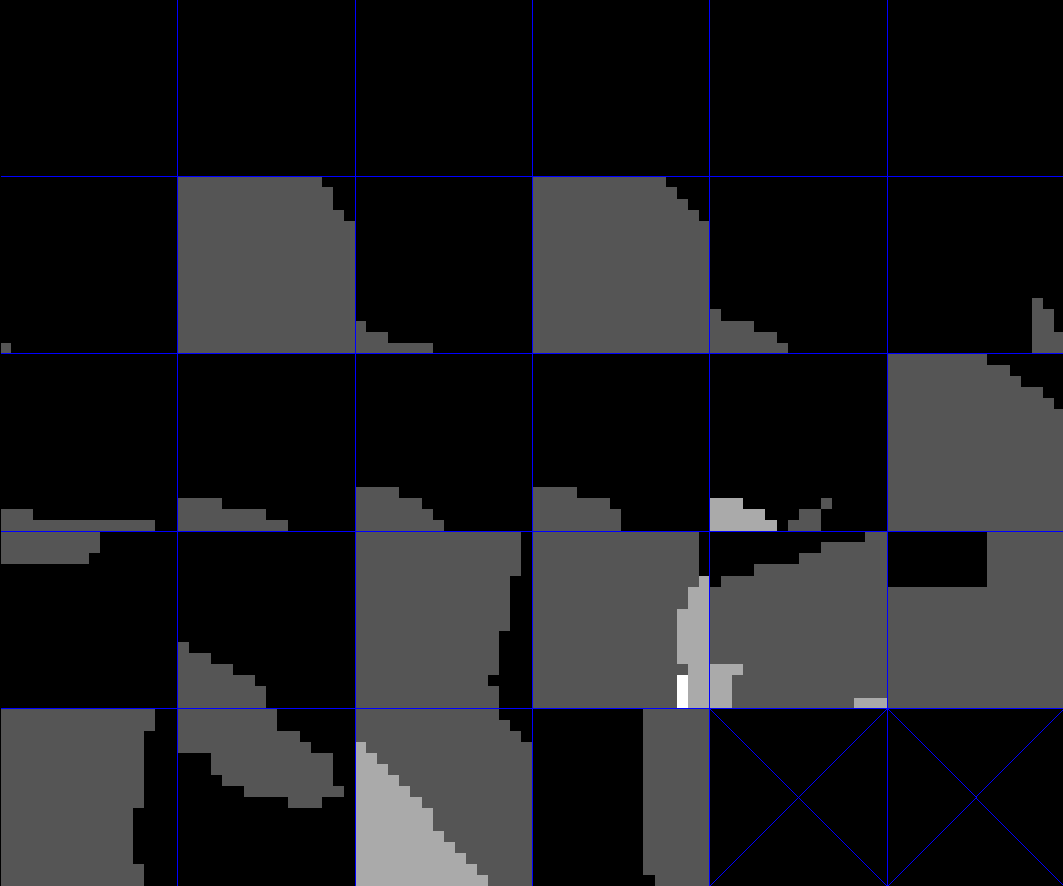
\includegraphics[width=0.45\textwidth]{images/srf/sf-leaf-segs.png}
  \label{fig:sf-leaf-segs}
 }
\caption[Inconsistency among the patches within a trained SF leaf]{{\bf Inconsistency} among the patches within a trained SF leaf. Notice that while the input patches (and consequently, the features computed based on them), are sufficiently similar, the same cannot be said about the segmentation patches. The {\bf representative prediction} is the medoid - upper left.}
\label{fig:srf-leaf}
\end{figure}

\begin{figure}[ht!]
\centering
 \subfigure[Decision tree inference]{%
  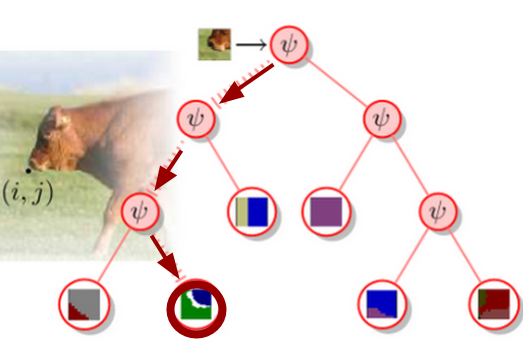
\includegraphics[width=0.57\textwidth]{images/srf/srf-tree-inference.png}
  \label{fig:srf-tree-inference}
 }
 \subfigure[Decision forest as an ensemble of multiple trees]{%
  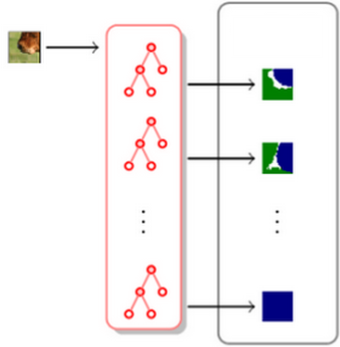
\includegraphics[width=0.4\textwidth]{images/srf/srf-inference-an-ensemble-of-trees.png}
  \label{fig:srf-inference-an-ensemble-of-trees}
 }
\caption{Inference with structured random forest. Images courtesy of~\cite{DollarBlog2013srf}}
\label{fig:srf-inference}
\end{figure}

\subsection{Edge detection}
\label{sec:ch2-edge-detection}
Now that a most-likely segmentation can be obtained given an input image patch, how to do edge detection on a whole image?

\subsubsection{Sliding window}
Structured labels capture information about entire pixel neighbourhood. Therefore a small number - $T$ of tree predictions per pixel suffice for high edge detection quality. Detection is performed by sliding a window across the image. The density of the sliding window is controlled by a parameter called {\it stride} $s = 2$ (a stride of $s = 1$ would mean that adjacent windows are considered). A set of $T$ trees are evaluated in a chequerboard-pattern (again, injecting randomness). So a total of $2T$ trees are trained. 

Each of the trees makes a prediction for the given location. For a patch side of $d = 16$, the locations in a $d$-neighbourhood are overlapping, and so are their predictions. With $T=4$, each pixel receives $\frac{T*d*d}{s*s}=256$ independent decisions.

% TODO show image with the intermediate result of just 4 trees averaged (the locations) - while that seems brittle, the added information from neighbouring overlapping patches helps denoise the predictions of the individual trees.

\subsubsection{Averaging of overlapping decisions}
The individual overlapping predictions %decisions 
are local segmentation masks. As discussed in \cref{Chapter1}, it is fairly easy to obtain an edge map, given a segmentation (see \fref{fig:segmentation}). This is how the multiple patches decisions have to be represented in order to aggregate the information in them for the purposes of edge detection. The combining is done by superimposing, %merging
and then averaging the edge maps from multiple overlapping patches. %decisions. 
This is referred to in the paper \cite{DollarICCV13edges} as a ``custom ensemble model''.

\section{Discussion}
At the time it was published, SE algorithm showed state-of-the-art performance on the now standard benchmark for the task of boundary detection - BPR on BSDS500~\cite{Arbelaez11}. The algorithm is tested on other datasets and the models learnt are capable of successfully finding edges in images from datasets that they were not specifically trained for. This is reassuring - it means that the detector is able to generalise - its knowledge is universal, instead of overly adapted to %fit for 
the contents of a specific dataset.

\settocdepth{section}
\subsection{An alternative way of capturing context}
\label{sec:ch2-alternative-capturing-context}
SE is not the only algorithm that detects edges while using local neighbourhood information.

\subsubsection{Oriented edge forests for edge detection}
\paragraph{Edge extraction}\mbox{}\\\mbox{}\\
A different approach is taken by Hallman and Fowlkes in their \textbf{Oriented edge forests (OEF)} paper \cite{Hallman2014} which was published towards the end of the current research work. They use a decision forest classifier to learn to distinguish between {\bf straight-line edges} of different {\bf position and orientation} within an image patch, see \fref{fig:OEF-oriented-patch-space}. Although they use a set of pre-defined edge classes, subsequent refinement of the edges (similar to the local {\it sharpening} introduced in \cite{Dollar2015PAMI}) % adds  a  subsequent  refinement  step  to  improve edge localisation.
helps them capture fine variations in edge shape and improves spatial localisation. OEF currently (as of February 2015) achieves best results on the BSDS500 benchmark.

\begin{figure}[ht!]
\centering
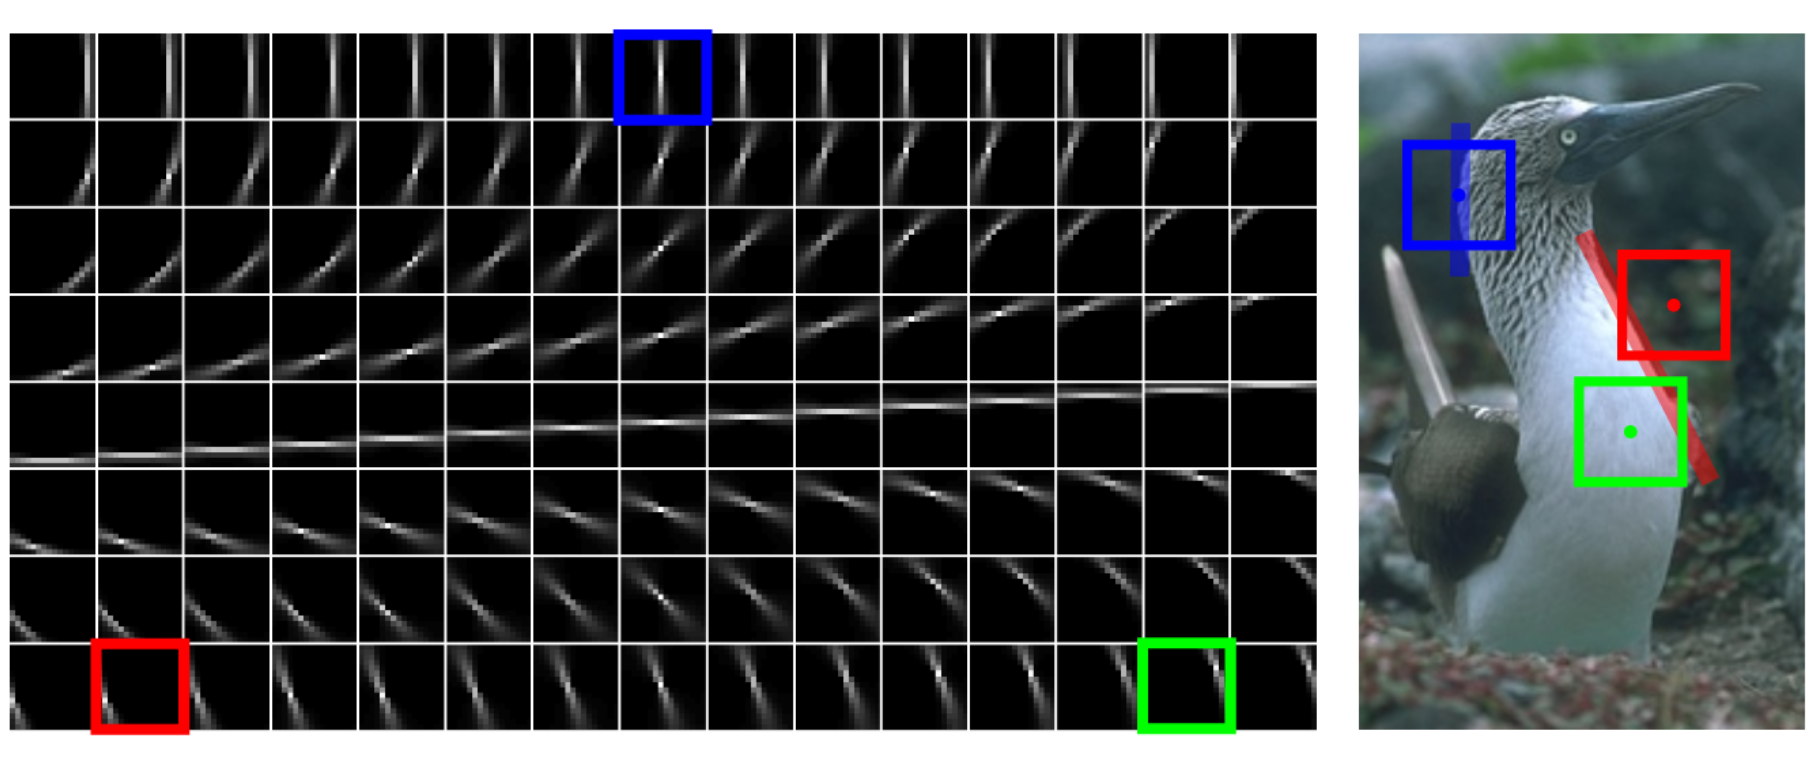
\includegraphics[width=0.8\textwidth]{images/OEF-oriented-patch-space.png} % not in srf/ subfolder as it is more ``related work''
\caption{Decision forest predicts a probability distribution over a fixed patch space (given on the left). Images courtesy of~\cite{Hallman2014}}
\label{fig:OEF-oriented-patch-space}
\end{figure}

\paragraph{OEF for image segmentation}
\subparagraph{Oriented probability of boundary}\mbox{}\\\mbox{}\\
The output of the OEF algorithm is an {\bf oriented probability of boundary} %(oPb)} 
$oPb(x,y,\theta)$. In their scenario, {\it oriented probability of boundary} means ``for a given angle $\theta$, what is the probability of having a {\bf straight-line edge} at (roughly) this angle''.

Another edge detector - gPb (for {\it global probability of boundary}) \cite{Maire2008using} also makes use of {\it oPb}. The OWT-UCM method, described in \cite{Arbelaez09} is a generic machinery which allows to create a hierarchy of segmentations out of any {\it oPb} detector output. The two ideas are combined in one pipeline: gPb-OWT-UCM \cite{Arbelaez11}, which we will discuss %describe 
in detail in \cref{Chapter3}. 

\subparagraph{OEF-OWT-UCM}\mbox{}\\\mbox{}\\
As already mentioned, OEF produces an {\it oPb}. It could therefore be expected that it would be a natural fit for the OWT-UCM algorithm. The resulting procedure, which Hallman \etal title ``OEF-OWT-UCM'' allows to use the edges extracted by OEF %edge detection results 
in order to obtain a hierarchical image segmentation. They report, however, misalignments due to quantisation mismatch of the orientation angles between their algorithm and gPb-OWT-UCM of \cite{Arbelaez11}.

\subsection{Limitations of SE}
While the SE algorithm is a state-of-the-art edge detector, it does not provide a segmentation. One still need to ``connect'' the resulting edges to extract complete contours. % that seem so obvious for the human eye+mind.

% TODO more drawbacks?

\subsection{Strong points of SE}
In our algorithm, which we will describe in \cref{Chapter4}, we choose to use {\it Structured edge} for edge extraction, as well as %and 
the {\it trained Structured forest}, for the following reasons:

{\bf SE}:
\begin{itemize}
 \item is an accurate edge detector,
 \item is fast at training time (which is carried out %done 
 offline),
 \item achieves real-time speed at test time - during edge detection,
 \item has potential as a general-purpose edge detector, %TODO add note - gPb seems to be highly-tuned for the BSDS500 dataset
 \item is able to predict a most-likely segmentation for a given input patch,
 \item can be augmented to store all those {\bf intermediate predictions} made during the edge extraction.
\end{itemize}

